\subsubsection{AIJ - Case A - Single building immersed in NSBL}
    \begin{figure}[h!]
        \centering
        \hypertarget{link:aij_A}{}
        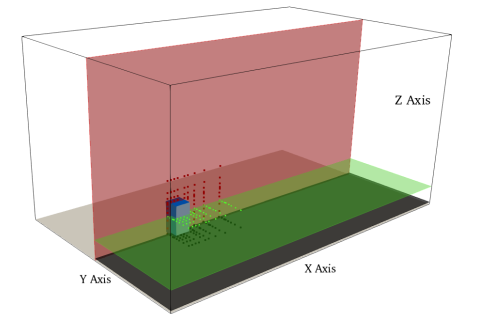
\includegraphics[scale=0.6]{imgs/aij_A.png}
        \caption{Single building immersed in NSBL}
    \end{figure}
    \textbf{Objectives:} 
    \begin{itemize}
        \item grid sensitivity analysis with steady state simulation (standard grid related analysis);
        \item from steady-state simulations to Scale Resolving Simulations (SRS), with kOmegaSSTSAS turbulence model, to highlight differences in terms of accuracy and computational cost (case-specific analysis);
        \item kOmegaSSTSAS turbulence model sensitivity analysis on the grid filter definition (case-specific analysis);
        \item SAS vs LES (case-specific analysis);
        \item development of Adaptive Mesh Refinement (AMR) criteria related to dispersion phenomena (methodology development);
        \item implementation of incremental POD for AMR (feature implementation);
        \item sensitivity analyses on turbulence models, numerical schemes, boundary conditions, and the effects of dimensionality reduction via intrusive ROM (validation-oriented study).
    \end{itemize}
    \textbf{Conclusions:} .... .\newline
